
\chapter{Reducing Runtime Overhead}

The identical function merging has no runtime penalty since it only alias two identical functions, removing one of the copies.
However, merging partially similar functions may introduce runtime overheads in a given execution path.

Figure~\ref{fig:partially-merged-blocks} shows an example of how function merging may introduce runtime overheads when merging two partially equivalent basic blocks.
The two basic blocks involved in this merge operation were extracted from the \texttt{462.libquantum} benchmark.
This example illustrates two different types of overheads that may be introduced during function merging:
$(i)$ the insertion of value selections;
$(ii)$ the insertion of branches to diverge to mismatching code or converge to matching code.


\begin{figure}[t]
  \centering
  \begin{subfigure}{\textwidth}
    \center
    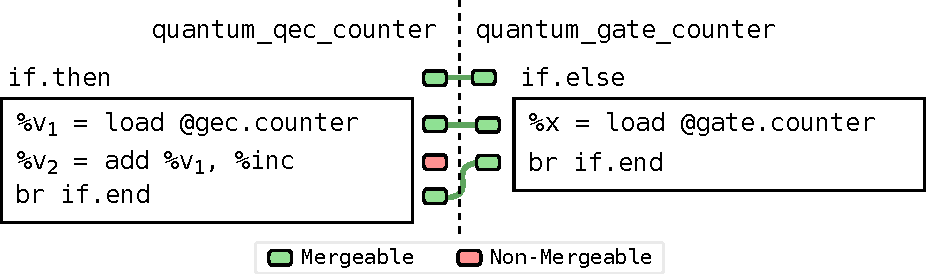
\includegraphics[scale=0.8]{src/runtime-overhead/figs/partially-merged-blocks-alignment}
    \caption{Pair of aligned basic blocks extracted from two larger functions in the \texttt{462.libquantum} benchmark.}
    \label{fig:partially-merged-blocks-alignment}
  \end{subfigure}
  \\
  \begin{subfigure}{\textwidth}
    \center
    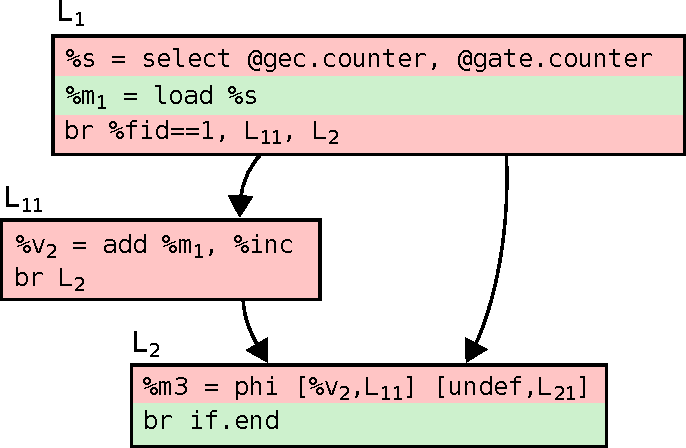
\includegraphics[scale=0.8]{src/runtime-overhead/figs/partially-merged-blocks-codegen}
    \caption{Merged code generated for the pair of aligned basic blocks.}
    \label{fig:partially-merged-blocks-codegen}
  \end{subfigure}
  \caption{Example of how function merging may introduce runtime overheads. }
  \label{fig:partially-merged-blocks}
\end{figure}

\section{Conservative Function Merging}\label{sec:conservative-fm}

In this section, we propose a conservative function merging approach that aims at minimal runtime overhead in the absence of profiling information.
The function merging approach described in Chapter~\ref{chap:fm-operation} is capable of partially merging basic blocks, inserting branches between instructions to split matching from non-matching code.
In order to minimise runtime overheads on possibly hot basic blocks, our conservative approach consider only merging whole basic blocks.

\section{Profile-Guided Function Merging}
